\subsection{What the detectors learn}\label{sec:shortcuts}
\paragraph{Cheap signals go a long way}
Table~\ref{tab:shortcuts} lists four shortcut indicators per corpus. The surface-statistics model recovers on average \StyleShare{} of the above-chance in-domain AUC of the full lexical model, and on the article corpora almost all of it (ISOT \StyleISOT, WELFake \StyleWEL). Sixty-four training examples are enough for an in-domain AUC of \LCsixfourISOT{} on ISOT and \LCsixfourWEL{} on WELFake; the claim and celebrity-headline corpora, whose in-domain scores are lower to begin with, learn much more slowly (LIAR \LCsixfourLIAR, GossipCop \LCsixfourGC). On the headline and claim corpora, publisher or speaker identity alone predicts the label with AUC \GroupPF{} (PolitiFact), \GroupGC{} (GossipCop) and \GroupLIAR{} (LIAR). A label that can be predicted from form, from a few dozen examples or from who published an item is a label whose in-domain score says little about veracity.

\begin{table}[t]
\centering
\caption{Shortcut indicators (ROC-AUC, mean of five seeds). In-domain AUC of \textsc{tfidf-lr} with the full training split, of the surface-statistics \textsc{style-gb}, and of \textsc{tfidf-lr} trained on only 64 or 256 items; AUC of a group-identity baseline (publisher domain for PolitiFact and GossipCop, speaker for LIAR); and the mean off-diagonal AUC with the corpus as source and as target.}\label{tab:shortcuts}
\small
\begin{tabular}{@{}lccccccc@{}}
\toprule
 & \multicolumn{5}{c}{in-domain} & \multicolumn{2}{c}{transfer} \\
\cmidrule(lr){2-6}\cmidrule(lr){7-8}
Corpus & full & style only & $n=64$ & $n=256$ & group only & as source & as target \\
\midrule
ISOT & 0.999 & 0.999 & 0.983 & 0.991 & -- & 0.611 & 0.670 \\
WELFake & 0.989 & 0.951 & 0.894 & 0.941 & -- & 0.626 & 0.540 \\
PolitiFact & 0.893 & 0.787 & 0.742 & 0.850 & 0.840 & 0.533 & 0.592 \\
GossipCop & 0.869 & 0.659 & 0.610 & 0.723 & 0.807 & 0.538 & 0.522 \\
LIAR & 0.698 & 0.590 & 0.567 & 0.607 & 0.664 & 0.537 & 0.530 \\
Twitter15 & 0.981 & 0.603 & 0.793 & 0.962 & -- & 0.572 & 0.563 \\
Twitter16 & 0.967 & 0.625 & 0.890 & -- & -- & 0.556 & 0.552 \\
\bottomrule
\end{tabular}
\end{table}


\paragraph{The strongest cues are collection signatures}
Figure~\ref{fig:weights} shows the highest-weight n-grams. In ISOT, the real class is signalled by Reuters wire conventions (``reuters'', ``said'', ``washington reuters'', weekday attributions such as ``on thursday'') and the fake class by the template of the sites it was collected from (``featured image'', ``image via'', ``read more'', ``video''). In WELFake, the real class is signalled by publisher suffixes inherited from one of its source collections (``breitbart'', ``york times'', ``mr'') and the fake class by the window in which fake items were gathered (``2016'', ``october'', ``november'', ``hillary''). Each corpus thus teaches a different, corpus-specific proxy, which explains why the sign of a cue can flip from one corpus to another (Section~\ref{sec:gap}).

\begin{figure}[t]
\centering
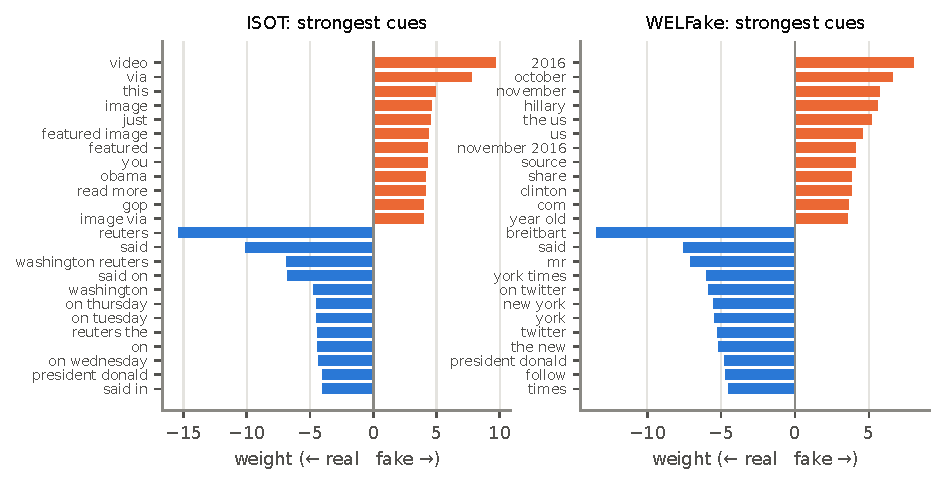
\includegraphics[width=\linewidth]{fig_weights}
\caption{Highest-weight n-grams of \textsc{tfidf-lr} (seed 0) for the real (blue) and fake (orange) classes. Both corpora are separated mainly by outlet conventions and collection-period vocabulary.}\label{fig:weights}
\end{figure}

\paragraph{Removing cues does not remove the signal}
Deleting the top-$K$ features and retraining barely moves in-domain AUC: on ISOT it goes from \TopKISOTIn{} with all features to \TopKISOTInThousand{} after deleting 1{,}000 and \TopKISOTInMax{} after 3{,}000, and on WELFake from \TopKWELIn{} to \TopKWELInThousand{} and \TopKWELInMax{}; transfer to the paired corpus, in contrast, falls from \TopKISOTPair{} to \TopKISOTPairMax{} (ISOT$\to$WELFake) and from \TopKWELPair{} to \TopKWELPairMax{} (WELFake$\to$ISOT). The highest-weight features thus carry most of what transfers, while the signal that keeps in-domain AUC near its ceiling is spread over thousands of corpus-specific features. Masking source tags, datelines, time expressions, numbers and named entities together (Table~\ref{tab:mask}) leaves in-domain AUC at \MaskISOTAllIn{} (ISOT) and \MaskWELAllIn{} (WELFake), and moves ISOT$\to$WELFake from \MaskISOTNonePair{} to \MaskISOTAllPair{} and WELFake$\to$ISOT from \MaskWELNonePair{} to \MaskWELAllPair{}. Balancing classes within each of 50 topic clusters, whose class purity averages \TopicISOTPurity{} in ISOT and \TopicWELPurity{} in WELFake, leaves in-domain AUC unchanged (ISOT \TopicISOTRandIn{}$\to$\TopicISOTBalIn{}, WELFake \TopicWELRandIn{}$\to$\TopicWELBalIn{}) and transfer unchanged (\TopicISOTRandOut{}$\to$\TopicISOTBalOut{}, \TopicWELRandOut{}$\to$\TopicWELBalOut{}); only GossipCop loses in-domain AUC (\TopicGCRandIn{}$\to$\TopicGCBalIn{}). The separating signal is therefore diffuse: it lives in style and register throughout the text, not in a removable list of tokens or topics, as \citet{verma2026audit} also found for ISOT.

\begin{table}[t]
\centering
\caption{Masking ablation (\textsc{tfidf-lr}, ROC-AUC, three seeds, first 3{,}000 characters). Rows: training corpus and what is masked in every corpus; columns: test corpus (the training corpus's own column is in-domain).}\label{tab:mask}
\small
\begin{tabular}{@{}llccccc@{}}
\toprule
Train & Masked & ISOT & WELFake & PolitiFact & GossipCop & LIAR \\
\midrule
ISOT & none & 0.998 & 0.679 & 0.739 & 0.481 & 0.559 \\
ISOT & source tags, datelines, URLs, handles & 0.997 & 0.681 & 0.733 & 0.483 & 0.559 \\
ISOT & dates, weekdays, numbers & 0.998 & 0.692 & 0.723 & 0.479 & 0.563 \\
ISOT & named entities & 0.996 & 0.657 & 0.678 & 0.543 & 0.557 \\
ISOT & all of the above & 0.996 & 0.650 & 0.678 & 0.540 & 0.556 \\
\addlinespace
WELFake & none & 0.808 & 0.980 & 0.636 & 0.529 & 0.532 \\
WELFake & source tags, datelines, URLs, handles & 0.815 & 0.979 & 0.634 & 0.533 & 0.536 \\
WELFake & dates, weekdays, numbers & 0.831 & 0.977 & 0.608 & 0.509 & 0.526 \\
WELFake & named entities & 0.833 & 0.965 & 0.614 & 0.511 & 0.522 \\
WELFake & all of the above & 0.810 & 0.964 & 0.611 & 0.500 & 0.522 \\
\bottomrule
\end{tabular}
\end{table}


\paragraph{Corpus divergence does not predict transfer}
Every pair of corpora can be told apart from text alone (proxy $\mathcal{A}$-distance between \PADmin{} and \PADmax{}, maximum 2; ISOT--WELFake \PADiw), yet across the 42 cells we find no association between source--target divergence and transfer AUC (Spearman $\rho=\PADrho$). With seven corpora the corpus-bootstrap 95\% interval is wide (\PADrhoCI), so a moderate association cannot be excluded, but label-free divergence is clearly not a usable predictor of transfer here. Transfer depends less on how different two corpora look than on whether the cue that separates the classes in one also separates them, with the same sign, in the other.
